\chapter{Lexikalische Markierungen}\label{lexikliji1}
 %\noindent
 Die folgende Analyse lexikalischer Markierungen strebt keine vollständige Beschreibung aller zu findenden Phänomene an, sondern will lediglich einzelne, besonders interessante und relevante Strategien sprachlicher Imitationen vorstellen, mit denen literaturjiddische Texte auf lexikalischer Ebene arbeiten.
 
 Eine Auswertung der Daten kann 
% nur
lediglich
 unter qualitativen Gesichtspunkten erfolgen. Komplexe quantitativ-statistische Analysen 
erlaubt das \isi{Korpus} kaum.
%  ist mit dem Korpus kaum möglich. %\todo{paraphrasiert}
 Dennoch wird versucht über die Tokenfrequenz bestimmter Phänomene quantitative Ergebnisse zu liefern. In Fällen lexikalischer Fragestellungen kann mit Hilfe von Frequenzklassen (\hai{{\FK}}),\footnote{Oft auch als \qu{logarithmic bins} oder \qu{Häufigkeitsklassen} bezeichnet.} basierend auf den Daten des \qu{Häufigkeitswörterbuch[s] gesprochener Sprache} (\citealt{Ruoff1981}), geprüft werden, ob ein frequenzbedingter Einfluss vorliegt. \citeauthor{Ruoff1981}s (\citeyear{Ruoff1981}) Daten zur deutschen Umgangssprache im Südwesten Deutschlands basieren auf dem Zwirnerkorpus.\footnote{Das unter der Leitung Eberhard Zwirnes zwischen 1955 und 1970 aufgebaute \isi{Korpus} von \qu{Schallaufnahmen aller deutschen Mundarten} ist über das Institut für Deutsche Sprache (\hai{IDS}) digital dokumentiert und zugänglich: \url{http://agd.ids-mannheim.de/download/korpus/Korpus_ZW_extern.pdf} [Stand: September 2014].} Ruoff berücksichtigt die Trennung nach Wortarten, die für die Berechnung der Tokenfrequenzen aufgehoben wurde. Dies ermöglicht zum einen den Vergleich mit \hai{{\FK}}n anderer Korpora, wie etwa denen des Deutschen Referenzkorpus (\hai{DeReKo}, 2012). Die Berechnung von Frequenzklassen erfolgt nach der Formel:\footnote{Die hier verwendete Formel folgt den Richtlinien des Institut für Deutsche Sprache (IDS) (\citealt[13]{DeReKo}). Die Gaußklammer bewirkt, dass das Ergebnis auf ganze Zahlen gerundet wird. Die Höhe des Ergebnisses bestimmt die Frequenzklasse.} 



\begin{center}\begin{math}
\hai{{\FK}} = \lfloor	log_2~ (\frac{Tokenfrequenz~des~untersuchten~Wortes}{Tokenfrequenz~des~häufigsten~Wortes}) + 0.5\rfloor 
\end{math}
\end{center} 
 

\largerpage
In Klasse 0 steht das häufigste Wort. Von 0 aufsteigend 
ist die \isi{Frequenz} pro Klasse abnehmend; d.\,h. Wörter der \hai{FK3} haben eine geringere Häufigkeit als Wörter der \hai{FK2}. Im Nenner der Formel zur Berechnung der \citeauthor{Ruoff1981}schen \hai{{\FK}}n steht der Wert 37536 für die Tokenfrequenz des häufigsten Lemma \sem{der/dieser} (vgl. \citealt[514–516]{Ruoff1981}). Die maximal erreichbare \hai{{\FK}} im \isi{Korpus} von \citealt{Ruoff1981} ist die \hai{FK15}. Das deutlich umfangreichere \hai{DeReKo} (2012) geht immerhin bis zur \hai{FK29} (vgl. Tabelle \ref{tblFKliji1} S.\, \pageref{tblFKliji1}). 

Zusätzlich werden an entsprechenden Stellen die \hai{{\FK}}n des Deutschen Referenzkorpus (\hai{DeReKo}) von 2012 herangezogen.\footnote{Die Berechnung der \hai{{\FK}}n erfolgt hier nach derselben Formel wie für \citealt{Ruoff1981}.} Das Diagramm in Abbildung \ref{ruoffderekofk} zeigt die Verteilung der in den Korpora vorhandenen Lemmata auf die einzelnen \hai{{\FK}}n.\footnote{Die diesem Diagramm zugrundeliegenden Einzeldaten sind in Tabelle \ref{tblFKliji1} S.\, \pageref{tblFKliji1} angeführt.} Man erkennt deutlich an der Kurve der Verteilung der \hai{{\FK}}n im \hai{DeReKo} (2012), die sich der Form einer Glockenkurve der Grundverteilung von \hai{{\FK}}n \,%rs keine Kommata
annähert. Lemmata mit einer hohen \isi{Frequenz} treten nur in geringer Menge auf. 
Beide Korpora zeigen eine Zunahme an Lemmata pro \hai{{\FK}}. Im umfangreicheren \hai{DeReKo} (2012) erkennt man eine steile Abnahme an Lemmata pro \hai{{\FK}} ab \hai{FK21}. Das \isi{Korpus} von \citealt{Ruoff1981} umfasst ein zu kleines Sample und reicht damit nur bis zu \hai{FK15}\,Lemmata mit niedrigeren Frequenzen sind also nicht belegt, was den Abbruch in der Graphik erklärt. Bis zu \hai{FK15} verhalten sich beide Korpora jedoch gleich. Ein Unterschied zwischen gesprochener (\citealt{Ruoff1981}) und geschriebener (\hai{DeReKo} 2012) Sprache zeigt sich betreffs der Menge an Lemmata pro \hai{{\FK}} nicht. \citealt{Ruoff1981} hat jedoch gegenüber dem \hai{DeReKo} (2012) den Vorteil einen älteren und dialektaleren Sprachstand zu repräsentieren. Aus diesem Grund wird letzteres nur zur Analyse allgemeiner Frequenzstrukturen angeführt, \citealt{Ruoff1981} jedoch als generelles Referenzkorpus verwendet. 

\begin{figure}
\begin{tikzpicture}
		\begin{axis}[width=0.95\textwidth,height=0.3\textheight,
		legend style={at={(1,1)},xshift=-9.25cm, yshift=-0.4cm,anchor=north west,nodes=left},
			%title={Textsorten des sp\"aten Westjiddisch},
			xtick={0, 5, 10,15,20,25},
			x tick label style={ /pgf/number format/1000 sep=}, 
			y tick label style={/pgf/number format/1000 sep=},
			%extra y ticks={456.1, 1022.4},
			extra y tick labels={1000,2000, 3000, 4000, 5000, 6000},
			extra y tick style={grid=major,
				tick label style={xshift=-1cm}},
				ymin=0.9,
			ylabel={Menge Lemmata pro \hai{{\FK}}},
			xlabel={\hai{{\FK}}},
			enlarge x limits=0.01]			
		
				
\addplot [dotted, very thick] table [x=FK, y=ruoff] {figures/FK_rouff.txt};
				
\addplot [color=black, thin] table [x=FK, y=dereko] {figures/FK_dereko.txt};
						
			\legend{Ruoff (1981), \hai{DeReKo} (2012)} %macht Legende
				
		\end{axis}
	\end{tikzpicture}
	\caption{Verteilung \hai{{\FK}}n bei Ruoff (1981) und \hai{DeReKo} (2012)}
	\label{ruoffderekofk}
	\end{figure}
	

 \section{Namen}\label{namenliji1}
 %\noindent

\largerpage
 Mit Blick auf die Namen der jüdischen Figuren der Korpustexte fällt auf, dass für männliche jüdische Figuren bestimmte Namen kennzeichnend sind (s. Tabelle \ref{tblnamenliji1}). Besonders populär sind Formen der Vornamen \textit{Moses}, \textit{Salomo}, \textit{Levy} und \textit{Isaak}. Aber auch die Stereotypenbezeichnung \qu{Jude} tritt wiederholt auf. 
  
\begin{table}[t]
	\begin{tabularx}{\linewidth}{lX}
	 \lsptoprule
	\textbf{Name} & \textbf{Beleg} \\ \midrule
\textit{Moses} & \textit{Moses} (\hai{FS}), \textit{Moses Herz} (\hai{EJ}), \textit{Schlaum Mosis} (\hai{DP}), \textit{Moses Posner} (\hai{PA}), \textit{Mauschel} (\hai{FL}) \\  \tablevspace

\textit{Salomo} & \textit{Salomon} (\hai{VE}), \textit{Schlaum Mosis} (\hai{DP}), \textit{Salomon Kraus} (\hai{JD}), \textit{Salomon Itzinger} (\hai{AB}) \\ \tablevspace

\textit{Levy} & \textit{Levi} (\hai{BS}, \hai{AH}), \textit{Lewy} (\hai{BP}), \textit{Herr Levin} (\hai{EV}), \textit{Meir Levi} (\hai{AD}) \\ \tablevspace

\textit{Isaak} & \textit{Isak} (\hai{AT}), \textit{Itzig} (\hai{DK}), \textit{Salomon Itzinger} (\hai{AB}), \textit{Itzick} (\hai{FL}) \\ \tablevspace%\textit{Veitel Itzig} \hai{SH} %sollundhaben	 
Namenlos & \textit{Jude} (\hai{LB}, \hai{PM}, \hai{PS},\hai{WA}, \hai{PF}) \\\tablevspace

einzeln auftretende \isi{Eigennamen} & \textit{Borig} (\hai{PL}), \textit{Lazarus} (\hai{FE}), \textit{Pinkus} (\hai{AO}), \textit{Ahasverus} (\hai{HJ}), \textit{Aaron Marcus Schleswicher} (\hai{TH}), \textit{Israel} (\hai{AJ}\,\hai{EJ}), \textit{Chailo} (\hai{AJ}), \textit{Moritz Kraus} (\hai{JD}), \textit{Bocham Mauksohn} (\hai{FM}), \textit{Ethan Lewenthaler} (\hai{FM}), u.\,a.\, \\ \lspbottomrule

	
	 		 \end{tabularx}
			\caption{Namen männlicher jüdischer Figuren im \hai{chrLiJi1}} \label{tblnamenliji1}
\end{table}

%\noindent Dieses Bild entspricht den populären Namen jüdischer Figuren in der deutschsprachigen Erzählliteratur zwischen 1918 und 1945, wie sie Frank \citeyear{Frank1987} herausarbeitet. Es zeigt damit, dass die Tradition typischer Namen für jüdische Charaktere bereits im 18. und 19. Jahrhundert zu den etablierten Mitteln der Figurenbildung zu rechnen ist.  

Die Belegdichte von Frauennamen ist sehr gering. Im Sample treten  keine vergleichbaren Erkennungsnamen, wie es bei den männlichen Figuren der Fall ist, auf. Es finden sich die Namen \textit{Rachel} (\hai{AJ} Berlin, 1825), \textit{Rebecke} (\hai{PF} Augsburg, 1816), \textit{Rosalie} (\hai{PF} Augsburg, 1816), \textit{Reichwerda Mauksohn} (\hai{FM} Leipzig, 1852), \textit{Sarah} (\hai{JD} Wien, 1866) oder auch nur das westjiddische Kennwort für \sem{Mutter} \textit{Memme} (\hai{DK} Osterwieck, 1872) (vgl. Abschnitt \ref{kennliji1}).


  \section{Kennwörter}\label{kennliji1}
%  %\noindent
Ein Hauptunterscheidungskriterium zwischen West- und \ili{Ostjiddisch} sind einige wenige Lexeme, bezüglich derer sich die beiden Varietäten unterscheiden. \textcite[1025]{Katz1983} zählt insgesamt elf dieser Lexeme, die \qu{entscheidende Isoglossen} zwischen Ost- und \ili{Westjiddisch} bilden.  \textcite[51]{AptrootGruschka2010} nennen noch drei weitere Lexeme. Tabelle \ref{tblkenn} führt die einzelnen Lexeme auf. Sie  können als \qu{Erkennungswörter} oder \qu{Schibboleths} der zwei Hauptvarietäten des Jiddischen verstanden werden. Die Wörter entstammen vorwiegend, aber nicht ausschließlich,\footnote{Zu nennen sind hier besonders Verwandtschaftsbezeichnungen wie jene für \sem{Großmutter}, \sem{Großvater}, \sem{Mutter} und \sem{Vater}, die auf germanische bzw. slawische Wurzeln zurück gehen; in einem Fall liegt aber auch ein Lexem romanischer Etymologie \,%rs ohne "h"
vor: \textit{oren} \sem{beten} < lat. \textit{orare}.} der hebräischen Komponente. 

\begin{table}[t]
\centering
	\begin{tabularx}{\linewidth}{XXX}
	\lsptoprule
\textbf{{\wj} Kennwort} & \textbf{{\oj} Kennwort} & \textbf{Bedeutung}\\ \midrule
\textit{éte} & \textit{táte} & \sem{Vater} \\
\textit{méme} & \textit{máme} & \sem{Mutter} \\
\textit{frále} & \textit{bóbe} & \sem{Großmutter} \\
\textit{hárle} & \textit{séyde} & \sem{Großvater} \\
\textit{mínich} & \textit{párve} & \sem{neutral gem. den jüd. Speisegesetzen} \\ 
\textit{ōrn} & \textit{dávenen} & \sem{beten} \\
\textit{óumern} & \textit{sfíre tseyln} & \sem{die 49 Tage von Pessach bis Schawout zählen} \\
\textit{pórschn} & \textit{tréjbern} & \sem{Fleisch von Sehnen reinigen} \\
\textit{sárgenes} & \textit{tachríkhim} & \sem{Totengewand} \\
\textit{schnōdern} & \textit{menáder sayn} & \sem{sich zu einer Spende verpflichten} \\
\textit{tretschn} & \textit{blosn shóyfer} & \sem{den Schofar blasen} \\
\textit{tfíle} & \textit{síder} & \sem{Gebetbuch} \\
\textit{trendl} & \textit{dreydl} & \sem{Kreisel} \\ \lspbottomrule

 \end{tabularx}
			\caption{Kennwörter des Ost- und Westjiddischen nach  \citealt[51]{AptrootGruschka2010}} \label{tblkenn}
\end{table}

Insgesamt zeigt sich im \isi{Korpus} eine gleichmäßige Verteilung an west- und ostjiddischen Kennwörtern. Es finden sich 13 Texte mit westjiddischen  und 14 Texte mit ostjiddischen Kennwörtern (s. Tabellen \ref{tblwjkennliji1} u. \ref{tblojkennliji1}). Allen voran stehen die Lexeme für \sem{Mutter} und \sem{Vater}. Dies mag damit zu erklären sein, dass dies hochfrequente Lexeme sind. Nach den Daten \citeauthor{Ruoff1981}s (\citeyear{Ruoff1981}) gehört \sem{Vater} zur \hai{FK6} und \sem{Mutter} zur \hai{FK7}.  
Demgegenüber ist \sem{beten} ein eher niedrigfrequentes Verb (\hai{FK11}), was den Wert der dieses Lexem verwendenden Quelle (\hai{OF} Frankfurt, 1711) erhöht. Das Ausbleiben von Belegen der Kennwörter für \sem{Großmutter} (\hai{FK11}) und \sem{Großvater} (\hai{FK10}) ist hingegen mit der geringen \isi{Frequenz} dieser Lexeme zu erklären. 
Andere Kennwörter wie {\oj} \textit{shoyferblosn}, {\wj} \textit{tretshn} \sem{den Shofar blasen} oder {\oj} \textit{sider}, {\wj} \textit{tfile} \sem{Gebetbuch}, sind Lexeme des jüdischen Kulturwortschatzes und  kaum von einem nicht-jüdischen Autor in höherer \isi{Frequenz} gebräuchlich.\footnote{Frequenzdaten zu diesen Lexemen existieren dementsprechend keine.} Der Umstand, dass keine weiteren Kennwörter belegt sind, mag also frequenzbegründet sein.
% für die bessere Lesbarkeit könnte man evtl. Leerzeichen bei den Aufzählungen einfügen

\begin{table}[t]
	\begin{tabularx}{\textwidth}{lX}
	\lsptoprule
\textbf{Kennwort} & \textbf{Beleg}\\ \midrule
\textit{Memme} \sem{Mutter} & \hai{BW} (112,116), \hai{LM} (24,28), \hai{AT} (90), \hai{GP} (7,8), \hai{PG} (13,15,53,61,63), \hai{JK} (25,26,28,29,34), \hai{NW} (33), \hai{DK} (44,45,46,47,48), \hai{PA} (62,64), \hai{UT} (Kap. 45), \hai{JP} (22R, 27, 52), \hai{FL} (39)\\ \tablevspace

\textit{Ette} \sem{Vater} & \hai{LM} (19,23,29), \hai{AT} (90), \hai{GP} (17), \hai{PG} (15,40,44,50,51), \hai{JK} (5,13,25, 26,28), \hai{JP} (5,18,21,22,23)\\ \tablevspace
\textit{oren} \sem{beten} &  \hai{OF} (3)\\ \lspbottomrule
 \end{tabularx}
    \caption{Westjiddische Kennwörter im \hai{chrLiJi1}} \label{tblwjkennliji1}
\end{table}

%\pagebreak 

\begin{table}[t]
	\begin{tabularx}{\linewidth}{lX}
	\lsptoprule
\textbf{Kennwort} & \textbf{Beleg} \\ \midrule
\textit{Tate} \sem{Vater} & \hai{BW} (112,\,116), \hai{NW} (28,\,30,\,125), \hai{PA} (63,\,64), \hai{DW} (67), \hai{SS} (9), \hai{LP} (38,\,39), \hai{GW} (3,\,9,\,15,\,17,\,18) \\ \tablevspace

\textit{Mamme} \sem{Mutter} & \hai{SS} (9), \hai{GW} (17,\,18,\,19,\,23)\\ \lspbottomrule


\end{tabularx}
			\caption{Ostjiddische Kennwörter im \hai{chrLiJi1}} \label{tblojkennliji1}
\end{table}


 
Es finden sich drei Texte, in denen westjiddische neben ostjiddischen Kennwörtern auftreten. In all diesen Fällen steht die westjiddische Form \textit{Memme} (\hai{BW} Leipzig, 1826:\,112,\, 116; \hai{NW} Berlin, 1804:\, 33; \hai{PA} Frankfurt, 1834:\, 62,\,64) neben der ostjiddischen Form \textit{Tate} (\hai{BW} Leipzig, 1826:\, 112,\,116; \hai{NW} Berlin, 1804:\, 28,30,125; \hai{PA} Frankfurt, 1834:\, 63,\,64). Zwei dieser Texte (\hai{BW} Leipzig, 1826 u. \hai{NW} Berlin, 1804) zeigen Reflexe des literarischen Diskurses: Solbrig (\hai{BW} Leipzig, 1826) hat den Autor Voß ( \hai{NW} Berlin, 1804) zum Vorbild, was sich auch bezüglich der verwendeten Manipulationsstrategien zeigt.

\newpage 
Das Histogramm in Abbildung \ref{kenn} verdeutlicht, dass das \isi{Korpus} bis in die 1870er Jahre keine Präferenzen für oder gegen westjiddische Kennwörter zeigt. Immerhin findet sich nach 1872 kein Beleg für westjiddische Speziallexik. Auch wenn die Datenmenge äußerst gering ausfällt, kann man dies als Hinweis auf den fortgeschrittenen \isi{Sprachtod} des Westjiddischen zum Ende des 19. Jahrhunderts deuten bzw. auf ein stärkeres Einfließen des Ostjiddischen. 

%%%Kennwörter
%\begin{flushleft}	
\begin{figure}[t]
	\begin{tikzpicture}
		\begin{axis}[only marks, width=0.82\textwidth,height=0.2\textheight,
		legend style={at={(1,1)},xshift=0.2cm, yshift=-0.5cm,anchor=north west,nodes=left},
			%title={Funktionstypen des sp\"aten Westjiddisch},
			xtick={1700, 1725, 1750, 1775, 1800, 1825, 1850, 1875, 1900, 1925, 1950}, ytick=\empty,
			x tick label style={/pgf/number format/1000 sep=}, 
			y tick label style={/pgf/number format/1000 sep=},
			%extra y ticks={456.1, 1022.4},
			%extra y tick labels={{456,1},{1022,4}},
			extra y tick style={grid=major,
				tick label style={, ,}},
				ymin=0.7,
				ymax=1.7,
			ylabel={Phänomenbelege},
			enlarge x limits=0.03]	
	
			
  			\addplot [mark=*, black] table [x=jahr, y=WJ] {figures/kennwoerterwj.txt};
 			\addplot [mark=o,black] table [x=jahr, y=OJ] {figures/kennwoerteroj.txt};

			% Andere Formen a={mark=square*,blue},% b={mark=triangle*,red},% c={mark=o,draw=black}}
						\legend{{\wj} Kennwörter, {\oj} Kennwörter} %macht Legende
		\end{axis}
	\end{tikzpicture}
	\caption{Kennwörter im \hai{chrLiJi1}}
	\label{kenn}	
\end{figure}
 




\begin{figure}[b]

 
	\begin{tikzpicture}
		\begin{axis}[only marks, width=0.66\textwidth,height=0.2\textheight,
		legend style={at={(1,1)},xshift=0.2cm, yshift=-0.03cm,anchor=north west,nodes=left},
			%title={Funktionstypen des sp\"aten Westjiddisch},
			xtick={1700, 1725, 1750, 1775, 1800, 1825, 1850, 1875, 1900, 1925, 1950}, ytick=\empty,
			x tick label style={/pgf/number format/1000 sep=}, 
			y tick label style={/pgf/number format/1000 sep=},
			%extra y ticks={456.1, 1022.4},
			%extra y tick labels={{456,1},{1022,4}},
			extra y tick style={grid=major,
				tick label style={, ,}},
				ymin=0.7,
				ymax=2.7,
			ylabel={Phänomenbelege},
			enlarge x limits=0.03]	
	
			 	\addplot [mark=o, black] table [x=jahr, y=kennostost] {figures/kennostregionOST.txt};%2.4
			 \addplot [mark=square] table [x=jahr, y=ojkenn] {figures/kennostregionWEST.txt};%2
			 \addplot [mark=*, black] table [x=jahr, y=Wjwesten] {figures/kennwjREGION_WEST.txt};%1.4
			 \addplot [mark=square*, draw=black] table [x=jahr, y=Wjosten] {figures/kennwjREGION_OST.txt};%1

			% Andere Formen a={mark=square*,blue},% b={mark=triangle*,red},% c={mark=o,draw=black}}
		      \legend{{\oj} Kennwörter im Osten, {\oj} Kennwörter im Westen, {\wj} Kennwörter im Osten, {\wj} Kennwörter im Westen} %macht Legende
		\end{axis}
	\end{tikzpicture}
 
	\caption{Regionale Verteilung von Kennwörtern im \hai{chrLiJi1}}
	\label{kennREGIONWJ}	

\end{figure} 


Um zu prüfen, ob ostjiddische Lexeme erst zu einem späteren Zeitpunkt ins westjiddische Gebiet eingedrungen oder dort schon länger präsent sind, wurde das Untersuchungsgebiet 
entlang des 9. Längengrads 
(Hamburg – Bregenz{;}\, vgl. S.\, \pageref{BregenzHH})  
in Ost und West unterteilt und jede Quelle einer dieser Regionen zugewiesen. 
Abbildung \ref{kennREGIONWJ} zeigt so zum einen, dass ostjiddische Kennwörter in nur zwei westlichen Quellen (aus Frankfurt) auftauchen. Diese Quellen zählen an sich nicht zu den ältesten aber auch nicht zu den jüngsten des Samples. Es ist prinzipiell nicht auszuschließen, dass in Frankfurt durch eine stärkere ostjiddische Migration Ost- und \ili{Westjiddisch} im 19. Jahrhundert parallel existierten (vgl. \citealt{Bertram1924}\,\citealt{AdlerRudel1959}\,\citealt{Maurer1986}\,\citealt[229–239]{Gay1994}). Ein sukzessives Einwirken ostjiddischer Formen auf den Westen ist tatsächlich nicht festzustellen. Das Histogramm in Abbildung \,%rs "Abbildung" ergänzen
\ref{kennREGIONWJ} zeigt uns, dass ein Gros der Belege westjiddischer Kennlexik aus dem östlichen Bereich unseres Untersuchungsgebiets stammt. Doch hier muss berücksichtigt werden, dass das Quellsample nur diachron, nicht diatopisch normalisiert wurde und so alle (!) räumlichen Strukturen, die sich daraus ablesen lassen, dem Zufall geschuldet sind. 


Die geographische Verteilung zeigt in den Dialektarealen des Westjiddischen überwiegend die Verbreitung westjiddischer Kennwörter (Abbildung \ref{kennkarte}). Ostjiddische Kennwörter treten  hingegen in der Nähe zum Ostjiddischen auf. Zwei Quellen entsprechen nicht diesem Bild: \hai{JK} (Breslau, 1810)  und \hai{PA} (Frankfurt, 1834). In \hai{JK} (Breslau, 1810) finden wir westjiddische Lexeme sehr weit im Osten des Untersuchungsgebietes, wo wir sie nicht erwarten würden. Im Fall von \hai{PA} (Frankfurt, 1834) ist Gegenteiliges der Fall, wo wir {\oj} \textit{Tate} (neben {\wj} \textit{Memme}) finden.  \,%rs "Memme" kursiv

\begin{figure}[]
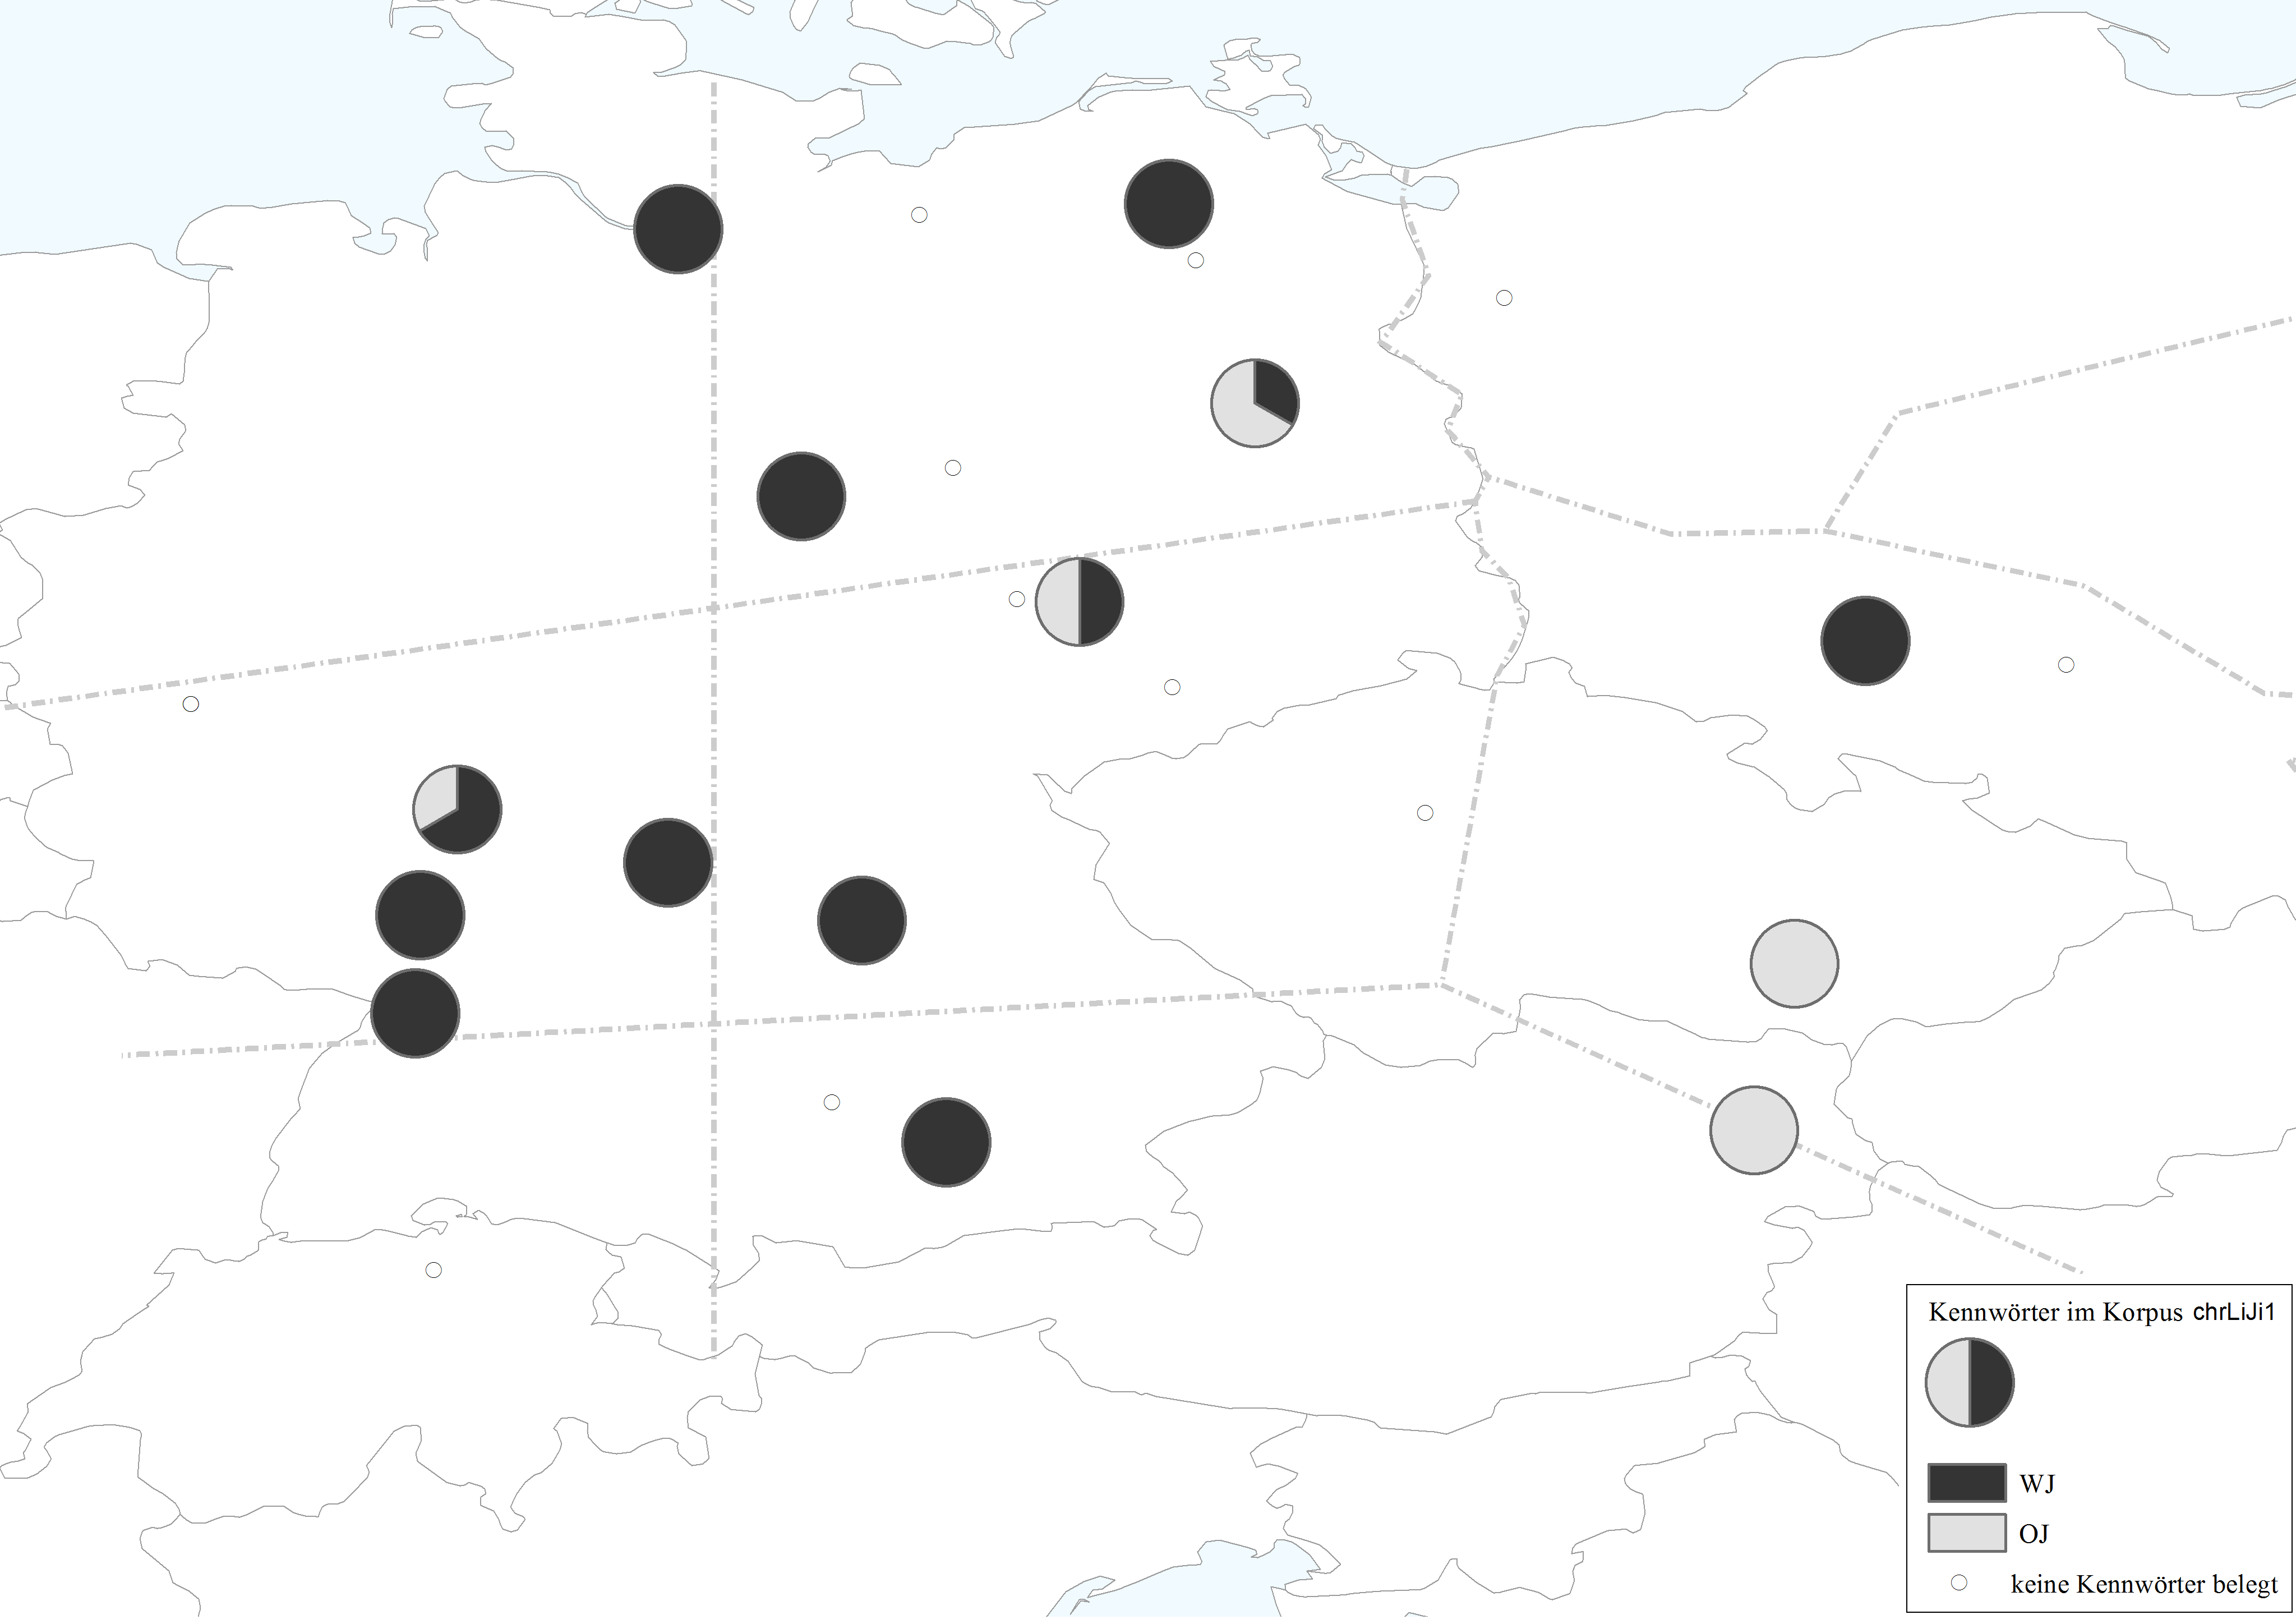
\includegraphics[width=\textwidth]{figures/kenn_diss.png}
\caption{\label{kennkarte} Kennwörter im \isi{Korpus} \hai{chrLiJi1}}
\end{figure} 
		


Eine der nur wenig bekannten innerwestjiddischen lexikalischen Variationen betrifft die Vokalisierung des \isi{Hebraismus}\il{hebräisch} \RL{שעה} \sem{Stunde}. Für das westliche \hai{{\SWJ}} ist die Form \textit{sche} belegt (\citealt[35]{GuggenheimGruenberg1976}\,\citealt[74]{Zivy1966}). Im \hai{{\NWJ}} hingegen findet sich die auch für das \hai{\OJ} übliche Form \textit{scho}. Wie genau diese binnenwestjiddische Isoglosse verläuft, ist leider nicht klar auszumachen, weil dieses Lexem für die relevanten Sprachräume des \hai{{\ZWJ}} und östl. \hai{{\SWJ}} nicht belegt ist. Im \hai{chrLiJi1} ist dieses Lexem in drei Fällen gegeben. In einer Quelle aus dem mitteldeutschen Raum findet sich sogar die aus dem Elsass und der Schweiz bekannte Form \textit{Scheh} \sem{Stunde} (\hai{OF} Frankfurt, 1711:\,1){;}\, als \textit{Scheih} findet sie sich in \hai{PG} (Speyer, 1835) (S.\,55) und die dem Ostjiddischen entsprechende Vokalisierung \textit{Schoh} ist in \hai{DG} (Wien, 1858) (S.\,14) belegt. In der Quelle \hai{PBreslau} des \hai{jüdLiJi1} findet sich ebenso die hier zu erwartende Form \textit{Schoh} (S.\,342).


Kennwörter, die lexikalische Unterschiede zwischen Ost- und \ili{Westjiddisch} markieren, sind im \hai{jüdLiJi1} nur wenige belegt. Westjiddische Lexeme treten keine auf, was auch mit Blick auf die geographische Lage der Quellen überraschend gewesen wäre. Statt dessen finden sich einige wenige ostjiddische Kennlexeme (Abbildung \ref{tblojkennjueliji1}).
 

\begin{table}
 
	\begin{tabular}{ll}
	\lsptoprule
\textbf{Kennwort} & \textbf{Beleg} \\ \midrule
 \textit{Tate} \sem{Vater} & \hai{GuS1} (3), \hai{GuS10} (9), \hai{PDebrecen} (7,\,14)\\
\textit{Mamme} \sem{Mutter} & \hai{GuS1} (3)\\ 
\lspbottomrule
\end{tabular}
			\caption{Ostjiddische Kennwörter im \hai{jüdLiJi1}} \label{tblojkennjueliji1}
\end{table}



      \section{Hebraismen}\label{hebrliji1}
%\noindent
Lexeme der \ili{hebräisch}-aramäischen\il{hebräisch} Komponente machen im (Surbtaler) Westjiddischen nach \citealt[45–49]
{GuggenheimGruenberg1976} einen Anteil von 2 bis 8\% aus. Im modernen Jiddisch sind es durchschnittlich 5\% des Wortschatzes \parencite[5f]{Timm2005}. Die tatsächliche Verwendung von Hebraismen ist jedoch stark von der Sprechsituation und Textsorte abhängig \parencite{Mark1954}. In beiden Varietäten machen Hebraismen jedoch im Allgemeinen nur einen äußerst geringen Anteil des Gesamtwortschatzes aus. 
 
Von 53 Quellen des \hai{chrLiJi1}-\isi{Korpus} setzen 44 Texte (83\%) Hebraismen zur Figurenmarkierung ein. Die Tokens variieren stark, was hauptsächlich der uneinheitlichen Textlänge geschuldet ist. Eine Frequenzuntersuchung gibt das \isi{Korpus} somit nicht her. Ich erlaube mir dennoch die sich rein auf den Leseeindruck stützende allgemeine Beobachtung, dass überwiegend Lexeme auftreten, welche Eingang in die deutsche Sprache gefunden haben (vgl. \citealt{Althaus2002,Althaus2004}). In sieben Quellen, in denen besonders viele und scheinbar der deutschsprachigen Mehrheit unbekannte (weil übersetzungbedürftige) Hebraismen eingesetzt werden, sind diese in Fußnoten oder einem Appendix übersetzt. Im überwiegenden Teil des \isi{Korpus} ist dies aber nicht der Fall und Hebraismen werden unübersetzt verwendet. Daraus lässt sich schließen, dass sie für Autor- wie Leserschaft als bekannt vorausgesetzt werden können.‏

  
Die rein qualitative Auswertung der Daten zeigt, dass bestimmte Types im intertextuellen Vergleich besonders häufig auftreten. Allen voran steht die Verwendung des Adjektivs \textit{meschugge} \sem{verrückt}, welches wir in 21 Quellen finden. Das entspricht 48\% der 44 Texte, in denen Hebraismen vorliegen. Ebenfalls relativ oft findet man die Lexeme \textit{Goi} \sem{Nichtjude} (in 12 Texten) und \textit{Schickse} \sem{Nichtjüdin} (in 10 Texten). Weitere 9\%–16\% der Quellen mit Hebraismen machen die in Tabelle \ref{tblhebrliji1} aufgeführten Types aus. 

\begin{table}
\centering
		\begin{tabularx}{\columnwidth}{lX}
	\lsptoprule
\textbf{Texte (\% von 44 Texten)} & \textbf{Type} \\ \midrule
 21 (48\%) & \textit{meschugge} \sem{verrückt}\\ %\midrule
12 (27\%) & \textit{Goi} \sem{Nichtjude} \\ %\midrule
 10 (23 \%) & \textit{Schickse} \sem{Nichtjüdin} \\ %\midrule
7 (16\%) &\textit{Dalles} \sem{Armut}, \textit{schmusen} \sem{sprechen} \\ %\midrule
6 (14\%) & \textit{dibbern} \sem{sprechen}, \textit{Reiwach}/\textit{Rewach} \sem{Gewinn}, \textit{koscher}/\textit{kauscher} \sem{(rituell) rein}\\ %\midrule
5 (11\%) & \textit{Massel} \sem{Glück}, \textit{Bonem}/\textit{Ponum} \sem{Gesicht}, \textit{acheln} \sem{essen}, \textit{Schaute}/\textit{Schoute} \sem{Narr}, \textit{Kapore} \sem{Verderben}, \sem{sterben}, \textit{Schama}/\textit{Schumme}/\textit{Schomme}  \sem{Seele}  \\ %\midrule
4 (9\%) &  \textit{Moos} \sem{Geld}, \textit{Schlamassel \sem{Unglück}}\\ \lspbottomrule

\end{tabularx}
			\caption{Häufige Hebraismen im \hai{chrLiJi1}} \label{tblhebrliji1}
\end{table}



Ein Großteil dieser Hebraismen sind Types, die in der deutschen Sprache eine hohe Tokenfrequenz haben. \textit{Verrückt} ist nach den Daten  \citeauthor{Ruoff1981}s (\citeyear[180]{Ruoff1981}) immerhin ein \isi{Adjektiv} der \hai{FK12} (\hai{FK7} innerhalb der Wortart). \textit{Sprechen} fällt in die \hai{FK9} der Verben, \textit{Glück} zählt zur \hai{FK10} (\hai{FK5} innerhalb der Wortart) und \textit{Gesicht} zur \hai{FK11} (\hai{FK6} innerhalb der Wortart) der Substantive \parencite[56, 55, 146]{Ruoff1981}. Die Grundfrequenz eines Lexems spielt also auch bei den Hebraismen eine Rolle.

Im \hai{jüdLiJi1} verwenden alle Texte der aufgenommenen \qu{Gedichte und Scherze in jüdischer Mundart} (\hai{GuS}) und alle Pamphlete, bis auf eine Ausnahme,\footnote{Die Ausnahme bildet \hai{PAlsleben}\,hier sind keine Hebraismen zu finden.} Hebraismen. Einige der im \hai{chrLiJi1} häufig auftretenden Types finden sich auch hier relativ oft (s. Tabelle \ref{tblhebrjuedliji1}), jedoch ist ein Vergleich der Korpora aufgrund des uneinheitlichen Textumfangs mit äußerster Vorsicht zu genießen. 

\begin{table}
\centering
	\begin{tabularx}{\textwidth}{lXX}\lsptoprule
\textbf{ Texte (\% von 10 Texten) } & \textbf{Type (Belegzahl \hai{GuS}:Pamphlete)} \\ \midrule
5 (50\%) & \textit{Goi} \sem{Nichtjude} (3:2)\\%\midrule
4 (40\%) & \textit{meschugge} \sem{verrückt} (2:2)\\%\midrule
3 (30\%) & \textit{koscher}/ \textit{kauscher} \sem{(rituell) rein} (2:1)\\%\midrule
2 (20 \%) & \textit{Schickse} \sem{Nichtjüdin} (2:0),  \textit{Kapore} \sem{Verderben}/ \textit{kapores} \sem{verderben}/ \sem{sterben} (1:1)\\%\midrule
1 (10\%) & \textit{schmusen} \sem{sprechen} (0:1), \textit{Ponim} \sem{Gesicht} (0:1), \textit{acheln} \sem{essen} (1:0)  \\
\lspbottomrule
\end{tabularx}
			\caption{Hebraismen im \hai{jüdLiJi1}} \label{tblhebrjuedliji1}
\end{table}




  \section{Interjektionen und psycho-ostensive Ausdrücke}\label{psycholiji1}
 %  %\noindent
Ein auffällig hoher Anteil der Texte arbeitet in der sprachlichen Markierung jüdischer Figuren mit Interjektionen und Phrasen des psycho-ostensiven Audrucks. 89\% (= 47 Texte) der Texte des \hai{chrLiJi1} \isi{Korpus} weisen diese Strategie auf. 

\subsection{Interjektionen}\label{interjektionen}
%  %\noindent
\largerpage
Ein interessantes Ergebnis ist, dass nicht viel Variation bei der Wahl der Interjektionen und Ausdrücke zu finden ist. Von orthographischen Alternativschreibungen abgesehen finden sich in den Texten die in Tabelle \ref{tblinterjektion} und exemplarisch in den Beispielen \ref{BSPinterjektion} aufgeführten Interjektionen. Allen voran steht die \isi{Interjektion} \textit{waih} \sem{wehe}, von der es mehrere Spielarten gibt (s. Tabelle \ref{tblwaih}). Gefolgt von der auch im Schriftdeutschen üblichen \isi{Interjektion} \sem{nun}. Die charakteristisch jiddischen Interjektionen \textit{oi} und \textit{nebbich} treten relativ selten auf (in insgesamt acht Texten vertreten). In einem Fall findet sich mit der eher aus dem oberdeutschen Raum bekannten \isi{Interjektion} \textit{mei} ein Einfluss der koterritorialen deutschen Dialekte (\ref{interjektmei}). Und auch die insgesamt sechs Belege für die \isi{Interjektion} \textit{ei} (\ref{interjektei}) kann Formen der Matrixsprache repräsentieren.

\begin{table}[t]
 
		\begin{tabular}{lccccccc}
	\lsptoprule
	\textbf{Interjektion} & \textit{waih} 	&   \textit{nu}, \textit{nü}  & \textit{ei}	&	\textit{oi} & \textit{nebbich}	& \textit{mei}	 \\ 
	& \sem{weh} & \sem{nun} & \sem{ei} & \sem{oh} & [unübersetzbar]\footnotemark & \sem{ja} \\ \midrule % horizontale Trennlinie
\textbf{Anzahl Texte} &	 36 & 25 & 6 & 3 & 3 & 1\\ \lspbottomrule
		 \end{tabular}
		 \caption{Interjektionen im \hai{chrLiJi1}}
		 \label{tblinterjektion}
		 \end{table}
		 
\footnotetext{Zu den verschiedenen Bedeutungen von \textit{nebbich} s. \citealt{Althaus1999}.}

\begin{table}[t]
 
		\begin{tabular}{lcccc}
			\lsptoprule
	\textbf{Interjektion} & \textit{au waih} & \textit{waih} 	&    \textit{waih geschrien}  & \textit{waih mer}	 \\ 
	& \sem{oh weh} & \sem{weh} & \sem{wehe geschrien} & \sem{wehe mir} \\ \midrule % horizontale Trennlinie
\textbf{Anzahl Texte} &	23 &  13 & 13 & 2 \\ \lspbottomrule
		 \end{tabular}
		 \caption{Varianten von \textit{waih} im \hai{chrLiJi1}}
		 \label{tblwaih}
		 \end{table}

 \eenumsentence{\label{BSPinterjektion}
\item \textit{O, waih mer, hot sich die ganze Welt} // \\
\textit{Auf einmol auf'n Kopf gestellt?!} (\hai{JP} Altona, 1867:\,15)\\\,%rs Absatz einfügen
	\sem{Oh weh mir, hat sich die ganze Welt auf einmal auf den Kopf gestellt?!}\label{interjektwai}

	\item \textit{Nü?! Worüm host Du mir gestaußen von Dir mit Antipäthie} (\hai{MV} Berlin, 1862:\,170)\\
	\sem{Na?! Warum hast du mich von dir mit Antipathie gestoßen}\label{interjektnu}


\item \textit{Ei hol dich der Teufel!} (\hai{AJ} Berlin, 1825:\,16)\label{interjektei}


\item \textit{Oi, a Broch!} (\hai{AK} Zürich, 1948:\,224)\\
	\sem{Oh, ein Fluch!}\label{interjektoi}
	
	\item \textit{Se wissen nichs, was is Nebbich? – Nebbich!} (\hai{GW} (n.a.,1900):\,4)\\
	\sem{Sie wissen nicht, was \textit{nebbich} ist? –\textit{Nebbich}!}\label{interjektnebbich}

	\item \textit{Mei, hab' ich doch oft die kleine Rosi auf meinen Armen getragen} (\hai{LP} Brünn, 1849:\,18)\\
	\sem{Ja, habe ich doch oft die kleine Rosi auf meinen Arm getragen}\label{interjektmei}

	
	}






 
In den Texten des \hai{jüdLiJi1} finden sich dieselben Interjektionen wie im \hai{chrLiJi1} (s. Tabelle \ref{tblwaihjüdliji}). In vier Quellen der \hai{GuS} findet sich \textit{nu}, in jeweils einer \textit{au mir},  \textit{ei weih} und  \textit{weih}. Die Pamphlete verwenden in jeweils zwei Texten \textit{weih geschriehn} und \textit{nu}. Es liegt damit, abgesehen von der \isi{Orthographie} des Diphthongs in \textit{waih} vs. \textit{weih}, kein Unterschied bei der Wahl der Interjektionen im Vergleich zu den Quellen des \hai{chrLiJi1} vor. 


\begin{table}
	
		\begin{tabular}{lccccc}
		\lsptoprule
	\textbf{Interjektion} & \textit{nu} & \textit{weih geschriehn}  & \textit{au mir} 	&    \textit{ei weih}  & \textit{weih}	 \\ 
	& \sem{nun} & \sem{wehe geschrien}& \sem{oh mir} & \sem{oh weh} & \sem{weh} \\ \midrule % horizontale Trennlinie
\textbf{Anzahl Texte} &	6 &  2 & 1 & 1 & 1 \\ \lspbottomrule
		 \end{tabular}
		 \caption{Interjektionen im \hai{jüdLiJi1}}
		 \label{tblwaihjüdliji}
		 \end{table}



   \subsection{Psycho-ostensive Ausdrücke}\label{psych}
  %  %\noindent
  Die in Unterabschnitt \ref{interjektionen} vorgestellten Interjektionen dienen vorrangig dem Ausdruck eines seelischen Zustandes des Sprechers. Darüber hinaus finden sich in den Korpora Phrasen des psycho-ostensiven Ausdrucks.  \textcite{Matisoff2000} fasst am Beispiel des modernen Ostjiddischen zwölf mögliche Subtypen dieser Ausdrücke zusammen, an denen sich die Analyse der Korpusdaten orientiert. Inwiefern das Jiddische einen besonderen Reichtum solcher Ausdrücke hat, wurde bislang noch nicht auf empirischer Grundlage bestätigt, es scheint aber im Allgemeinen als \textit{Mythos} dem Jiddischen anzuhängen (vgl. \citealt[4]{Matisoff2000}). 
  
In den Texten des \hai{chrLiJi1} finden \,%rs Pluralbezug
sich die in Tabelle \ref{tblpsych}  aufgeführten Typen, die hier mit allen erhobenen Belegen versehen sind. Es überwiegen senderbezogene Äußerungen gegenüber empfängerbezogenen, was sicherlich auf die literarische Rolle der jeweiligen Judenfiguren als weitestgehend isolierte Gegenspieler zurückzuführen ist. 

  \begin{table}[t]
%\centering
		\begin{tabularx}{\columnwidth}{lX}
		\lsptoprule
	Typ & Beleg	 \\ \midrule % horizontale Trennlinie
	

allo-bono-petitive & \textit{daß sie sollen hundert Johr leben!} (\hai{DW}:\,69){;}\,  \textit{Gott behüt se} (\hai{FE}:\,16){;}\, \isi{Eigennamen} \& Verwandtschaftsbezeichnungen mit \textit{-leben}:  \textit{Bohlmannleben} (\hai{DP}:\,5), \textit{Mosisleben} (\hai{DP}:\,15), \textit{Kinderleben} (\hai{JP}:\,5, 19),  \textit{Sorcheleben}  (\hai{JP}:\,17R),  \textit{Memmeleben} (\hai{JP}:\,22R),  \textit{Etteleben} (\hai{JP}:\,52),  \textit{Doktorleben} (\hai{SS}:\,12),  \textit{Inspektorleben} (\hai{SS}:\,13),  \textit{Herrgottleben} (\hai{SS}:\,25),  \textit{Rebbeleben} (\hai{SS}:\,26{;}\, \hai{GW}:\,19), \textit{Rüfkeleben} (\hai{GW}:\,10), \textit{Mutterleben} (\hai{GW}:\,10), \textit{Meierleben} (\hai{GW}:\,12), \textit{Narreleben} (\hai{GW}:\,12), \textit{Direktorleb'm} (\hai{GW}:\,12), \textit{Schmulleben} (\hai{GW}:\,14), \textit{Tateleben} (\hai{GW}:\,15), \textit{Jankefleben} (\hai{GW}:\,32). \\
% \tablevspace
auto-bono-petitive & \textit{soll ich leben} (\hai{JP}:\,24). \\
% \tablevspace
auto-malo-fugitive & \textit{Gott soll hüten} (\hai{SS}:\,19), \textit{Gott behit} (\hai{AT}:\,88, 89, 90, 109){;}\, \textit{Gott soll mich bewohre} (FE:\,\hai{14}), \textit{Gott soll me schamer seyn} (\hai{FE}:\,56), \textit{Soll mir Gott helfen} (\hai{FS}:\,40, 42), \textit{Gott soll schützen!} (\hai{AJ}:\,1, 2, 6, 10), \textit{Gott soll mir helfen!} (\hai{AJ}:\,1), \textit{Gott soll mer helfen} (\hai{PF}:\,9, 21), \textit{Soll mir Gott helfen} (\hai{PM}:\,212, 218).\\ 
% \tablevspace
auto-malo-recognitive & \textit{waih mir} (\hai{JP}:\,15, 42), \textit{Wey mir!} (\hai{AO}:\,85){;}\, \textit{nebbisch} (\hai{SS}:\,13), \textit{nebech} (\hai{DG}:\,6), \textit{nebbich} (\hai{GW}:\,4,5,10){;}\, \textit{was thu ich damit!} (\hai{NW}:\,11), \textit{was thu’ ich damit!} (\hai{EV}:\,279), \textit{Was duh ich domit?} (\hai{TH}:\,98), \textit{was thut mer damit?} (\hai{EJ}:\,38){;}\, \textit{mahn Seel} (\hai{SV}:\,4), \textit{meine Schama} (\hai{LP}:\,41), \textit{meine Schumme} (\hai{OF}:\,2), \textit{man'neschommæ} (\hai{LR}:\,6). \\
% \tablevspace
auto-bono-recognitive & \textit{Gotts Wunder} (\hai{PF}:\,12, 17, 19), \textit{Gottes Wunder} (\hai{LP}:\,14), \textit{Gotteswunder} (\hai{LP}:\,15).
 \\\lspbottomrule

		 \end{tabularx} 
		 \caption{Psycho-ostensive Ausdrücke im \hai{chrLiJi1}}
		 \label{tblpsych}
		 \end{table}   
  % \clearpage
   
   
   
 Das \hai{jüdLiJi1} zeigt deutlich weniger solcher Ausdrücke. Lediglich in drei Belegen liegen auto-malo-fugitive (\ref{fugitivjuedliji1}) und auto-bono-petitive Ausdrücke (\ref{petitivejuedliji1}) aus der Quelle \hai{PBerlin1} vor:
 \eenumsentence{
	\item \textit{soll mer Gott helfen} \\
	\sem{soll mir Gott helfen} (\hai{PBerlin1}:\,2, 6)\label{fugitivjuedliji1}

	\item \textit{soll ich leben} (\hai{PBerlin1}:\,4)\label{petitivejuedliji1}

	
	}
     
 Die geringe Belegzahl an psycho-ostensiven Ausdrücken im \isi{Korpus} des \hai{jüdLiJi1} ist jedoch kein Indiz dafür, dass solche Ausdrücke im gesprochenen Westjiddischen kaum verbreitet waren. Zumindest das westjiddische Theaterstück \quji{\RL{דיע ה{א\makebox(-1.25,-1.25)[r]{\libertineGlyph{uni05B8}}}כצייט צו גר{א\makebox(-1.25,-1.25)[r]{\libertineGlyph{uni05B8}}}בסד{א\makebox(-1.25,-1.25)[r]{\libertineGlyph{uni05B8}}}רף}} [\qu{Die Hochzeit zu Grobsdorf}] (1822) gebraucht solche Ausdrücke besonders häufig, wie die Beispiele in (\ref{psychgrob}) zeigen.
 \eenumsentence{\label{psychgrob} \,%rs Absätze zwischen Zitierform und Übersetzung 
 	\item  \RL{איבער הונדערט י{א\makebox(-1.25,-1.25)[r]{\libertineGlyph{uni05B8}}}הר} \\
    \sem{über hundert Jahre (soll er alt werden)} allo-bono-petitive\\
    (\qu{Die Hochzeit zu Grobsdorf} 1822:\,13)\footnote{Die Seitenangaben folgen der Seitennummerierung der Handschrift aus der Max Weinreich Collection (Sig.: RG 584), auf welchem die Jahresangabe \qu{1822} zu finden ist.} 
    
	\item \RL{נ{א\makebox(-1.25,-1.25)[r]{\libertineGlyph{uni05B8}}}ך הונדערט קינדער}\\
    \sem{noch hundert Kinder (soll ich bekommen)} auto-bono-petitive\\
    (\qu{Die Hochzeit zu Grobsdorf} 1822:\,14) 
 
 	\item \RL{מיינע שמה}\\ 
    \sem{meine Seele} auto-malo-recognitive\\
    (\qu{Die Hochzeit zu Grobsdorf} 1822:\,u.\,a.\, 6,16,20,21,22) 
 }

Allgemein lässt sich festhalten, dass jüdische Figuren in allen Stadien des \hai{{\LiJi}} über besondere Ausdrücke entwickelt werden, die den psychischen Zustand des Sprechers ausdrücken.
Tatsächlich sind solche Ausdrücke für die (west-)jiddische Sprachrealität dokumentiert vgl. Bsp. in (\ref{psychgrob}). Ob sie jedoch mit der \isi{Frequenz}, wie wir es im \hai{chrLiJi1} finden, auch in der gesprochenen Sprache verwendet wurden, muss offen bleiben. Der hohe Gebrauch von Interjektionen im \hai{chrLiJi1} spricht dafür, dass diese, allen voran Variationen mit \textit{waih}, auch im literarischen Diskurs als besondere Kennzeichen jüdischer Figuren dienen.

\section{Gallizismen}\label{galliliji1}
%\noindent
Im Bereich der Lexik sei noch ein letztes Phänomen näher beleuchtet. Stark verbunden mit dem \qu{Juden-Französisch-Deutsch} \parencite[175]{Gelber1986} (s. Unterabschnitt \ref{assimiliert}) ist die Verwendung von Gallizismen im \hai{chrLiJi1}.
Die in (\ref{bspgall}) aufgeführten Belege zeigen, dass keine bestimmten Lexeme besonders häufig auftreten, wie es im Fall der Interjektionen und psycho-ostensiven Ausdrücken gegeben ist (Abschnitt \ref{psycholiji1}). Unter den Gallizismen sind einige, die bereits in das System der Matrixsprache integriert sind z.\,B.\, (\ref{mammsellchen}), (\ref{arretueren}) und damit nicht zwangsläufig als Produkte der sprachlichen Manipulation gewertet werden müssen. 

\eenumsentence{

	\item\textit{l’age} \sem{Alter} (\hai{BW} Leipzig, 1826:\,101)
\item\textit{par tout} \sem{um jeden Preis}  (\hai{PL} Mannheim, 1780:\,41)
\item \textit{Cavaliers} \sem{Kavalliere} (\hai{DW} Wien, 1773:\,71)
\item \textit{Dames} \sem{Frauen} (\hai{DW} Wien, 1773:\,71{;}\, \hai{PA} Frankfurt, 1834:\,5)   
\item\textit{Trän} \sem{Zug} (\hai{PM} Magdeburg, 1792:\,219)
\item\textit{Plaisir} \sem{Freuden} (\hai{FS} Schwerin, 1805:\,41)
\item \textit{wollt ich gern seyn content} \sem{ich möchte zufrieden sein} (\hai{FS} Schwerin, 1805:\,42)
\item\textit{Malleur} \sem{Unglück} (\hai{TH} Merseburg, 1820:\,115){;}\, \textit{malheur} \sem{Unglück} (\hai{AD} Leipzig, 1846:\,135)
\item \textit{Mamsellchen} \sem{Fräulein} (\hai{TH} Merseburg, 1820:\,122)\label{mammsellchen}
\item \textit{foi de parol} \sem{Wort des Glaubens} (\hai{AJ} Berlin, 1825:\,2)   
\item\textit{arretüren} \sem{festnehmen} (\hai{AB} Hamburg, 1850:\,47)\label{arretueren}
\item\textit{fête} \sem{Fest} (\hai{AD} Leipzig, 1846:\,136)
  }\label{bspgall}

Die Markierung funktioniert nicht über die Lexeme selbst, sondern allein über die Wahl der Sprache. Dabei treten in den meisten Fällen nur einzelne Lexeme innerhalb des \hai{{\LiJi}} auf, keine Sätze oder Phrasen. Einzige Ausnahme ist dabei Sessas Stück \hai{JK} (Breslau, 1810), in dem die jüdische Hauptfigur mit einem französischen Soldat \ili{französisch}, bzw. \qu{Juden-Französisch-Deutsch} \parencite[175]{Gelber1986}, spricht: \\

\eenumsentence{

	\item\textit{Qui, qui, nous sommez des pauvres Juifs, amix von där graußen Nation.}\\
	 (\hai{JK} Breslau, 1810:\,37–38)\\
	\sem{Wer, wer{;}\, wir sind arme Juden, Freunde von der großen Nation.}
}\label{galljk}
   
Die elf\, Texte, in denen wir Gallizismen finden, streuen diachron interessant. Nach 1850 bricht diese Strategie der Figurencharakterisierung ab (s. Abbildung \ref{gall}). 

%%%Gallizismen%\begin{flushleft}	
\begin{figure}
	\begin{tikzpicture}
		\begin{axis}[only marks, width=0.82\textwidth,height=0.2\textheight,
		legend style={at={(1,1)},xshift=+0.2cm, yshift=-0.25cm,anchor=north west,nodes=left},
			%title={Funktionstypen des sp\"aten Westjiddisch},
			xtick={1700, 1725, 1750, 1775, 1800, 1825, 1850, 1875, 1900, 1925, 1950, 1975}, ytick=\empty,
			x tick label style={/pgf/number format/1000 sep=}, 
			y tick label style={/pgf/number format/1000 sep=},
			%extra y ticks={456.1, 1022.4},
			%extra y tick labels={{456,1},{1022,4}},
			extra y tick style={grid=major,
				tick label style={, ,}},
				ymin=0.7,
				ymax=2.5,
			ylabel={Phänomenbelege},
			enlarge x limits=0.03]	
	%TT problem?
			
		\addplot [mark=*, black] table [x=jahr, y=gall] {figures/gall.txt};
	\addplot [mark=o, black] table [x=jahr, y=no] {figures/gall_no.txt};

			% Andere Formen a={mark=square*,blue},% b={mark=triangle*,red},% c={mark=o,draw=black}}
						\legend{Gallizismen, übrige Quellen} %macht Legende
		\end{axis}
	\end{tikzpicture}
	\caption{Gallizismen im \hai{chrLiJi1}}
	\label{gall}	
\end{figure}
 %TT no-Belege aufführen!

   
Dieses Phänomen ist auf das \hai{chrLiJi1} beschränkt. Im \hai{jüdLiJi1} spielen Gallizismen keine Rolle. Es ist eindeutig ein pejoratives Element des \hai{chrLiJi1} und hat keine Entsprechung in autochthonen Quellen des Westjiddischen. Gallizismen tragen zum einen die Funktion, den Multilingualismus und damit unter pejorativer Verwendung den Mythos eines \textit{globalen jüdischen Verschwörungsnetzwerks} zu vermitteln. Zum anderen aber verbindet die gezielte Verwendung des Französischen das Feindbild \textit{Franzose} mit dem Feindbild \textit{Jude} (vgl. Abschnitt \ref{assimiliert}, S.\, \pageref{judenfranzoesischdeutscherstmals}). 